% ============================================================
%  Rozdział 4 — PKP: Prędkość, Kąt, Przechył
% ============================================================
\section{PKP — Prędkość, Kąt, Przechył}

Najbardziej istotne elementy przy większości manewrów — szczególnie przy wchodzeniu
i wychodzeniu z cofki — to \textbf{P}rędkość, \textbf{K}ąt i \textbf{P}rzechył.

\begin{description}[leftmargin=1.5em, style=nextline, font=\bfseries]

  \item[Prędkość]
    Pozwala na przecięcie hyżki. Bez odpowiedniej prędkości wyjście z cofki jest niemożliwe — hyżka zabiera dziób kajaka i obracamy się w miejscu.

  \item[Kąt]
    Pozycja kajaka w stosunku do hyżki. Pomaga lub utrudnia przecięcie hyżki i decyduje o tym, w jakiej pozycji kajak znajdzie się po wykonaniu manewru. Odpowiedni kąt zależy
    też od siły nurtu — im mocniejszy nurt, tym ostrzejszy kąt.

  \item[Przechył]
    Pomaga ustabilizować i kontrolować kajak. Powinien być mały, ale stabilny. Zasada: \textbf{DUPA DO NURTU} — nurt zawsze powinien napierać na krawędź znajdującą
    się wyżej, najlepiej w dno kajaka.

\begin{figure}[H]
    \centering
    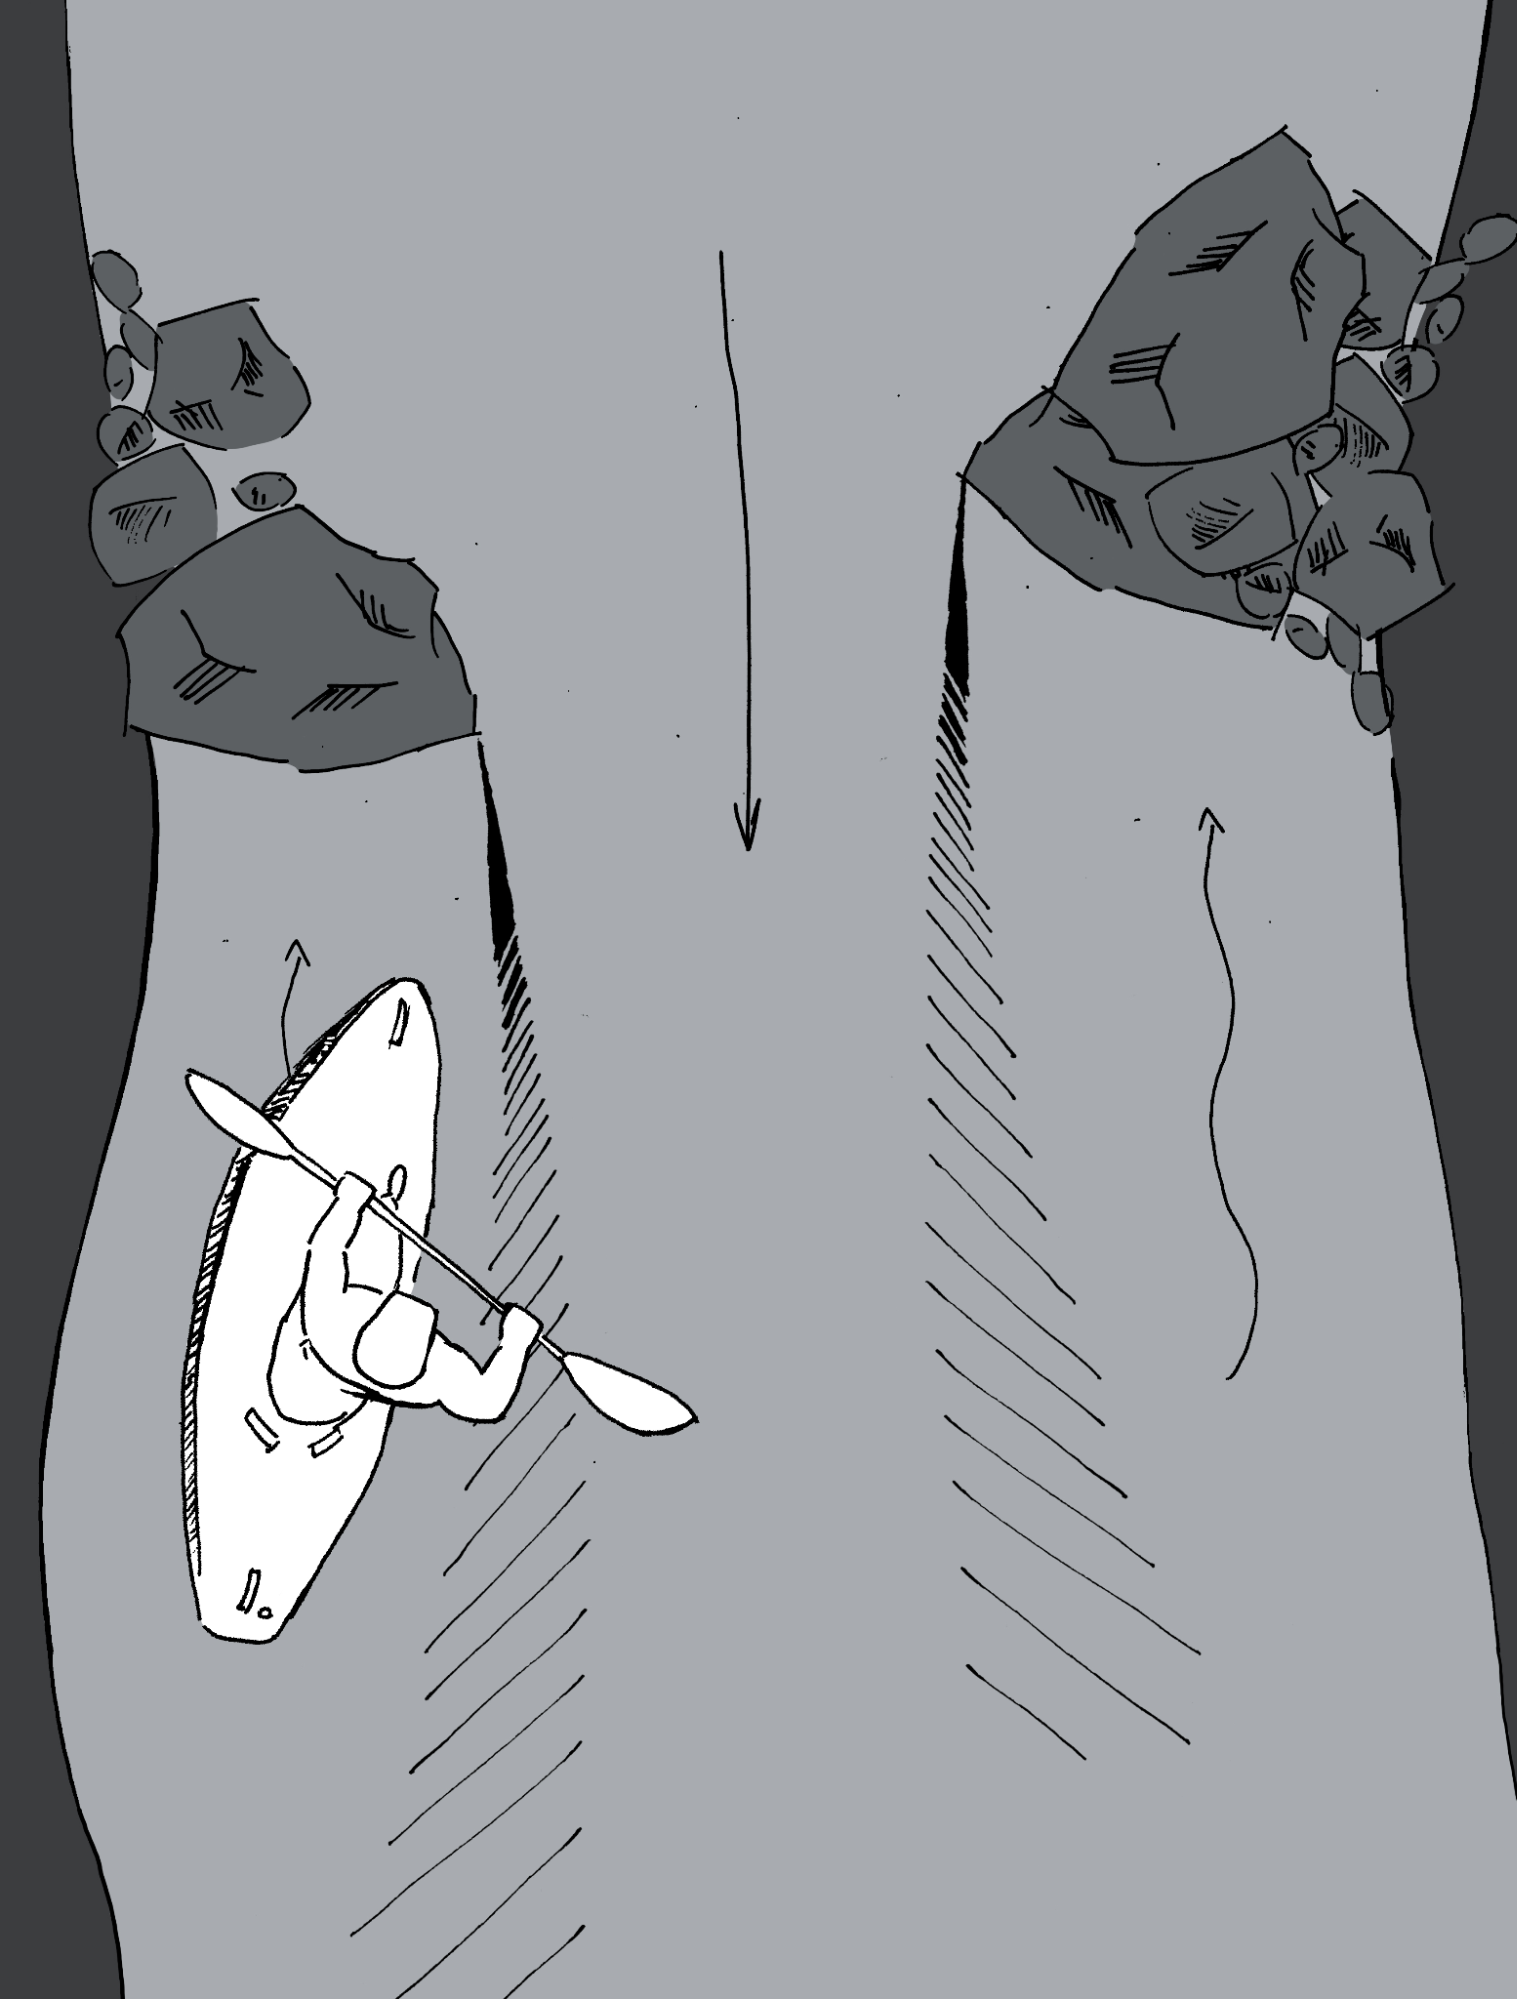
\includegraphics[width=300px]{images/wyjscie_na_nurt.png}
    \caption{Schemat wychodzenia na nurt}
\end{figure}

\end{description}
